%\documentclass[crop,tikz,convert={outext=.svg,command=\unexpanded{pdf2svg \infile\space\ou
%tfile}},multi=false]{standalone}[2012/04/13]

\documentclass[crop,tikz]{standalone}[2012/04/13]


\newcommand{\pd}[2]{\frac{\partial #1}{\partial #2}}
\usepackage{pgf}

\usetikzlibrary{arrows,automata}
\usepackage[latin1]{inputenc}
\begin{document}
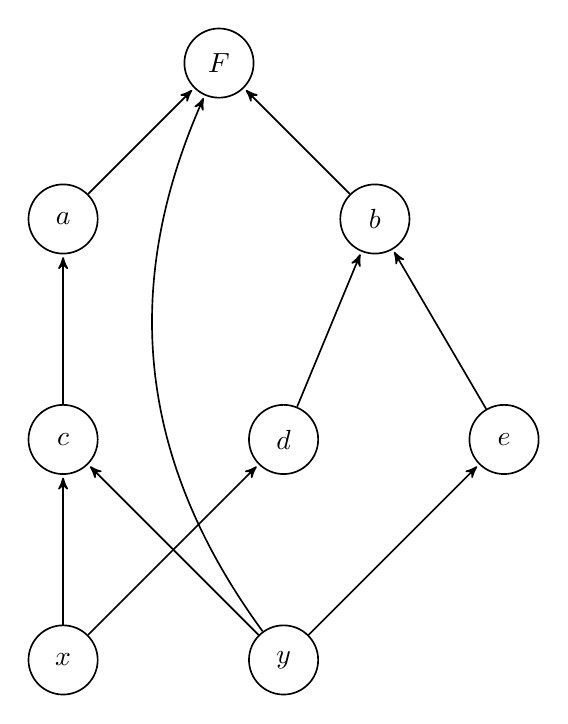
\begin{tikzpicture}[->,>=stealth',shorten >=1pt,auto,node distance=2.8cm,
                    semithick]
 % \tikzstyle{every state}=[fill=red,draw=none,text=white]

  \node[state]         (A)                    {$F$};
  \node[state]         (B) [below left of=A] {$a$};
  \node[state]         (C) [below right of=A] {$b$};
  \node[state]         (D) [below of=B]       {$c$};
  \node[state]         (E) [right of=D] {$d$};
  \node[state]         (F) [right of=E]       {$e$};
  \node[state]         (G) [below of=D]       {$x$};
  \node[state]         (H) [right of=G]       {$y$};
  

  
  \path (B) edge              node {} (A);
  \path (C) edge              node {} (A);
  \path (E) edge              node {} (C);
  \path (F) edge              node {} (C);
  \path (D) edge              node {} (B);
  \path (G) edge              node {} (D);
  \path (G) edge              node {} (E);
  \path (H) edge              node {} (D);
  \path (H) edge              node {} (F);
  \path (H) edge [bend left]  node {} (A);
\end{tikzpicture}

\end{document}